At the beginning of this document, I set out to explore the following thesis:

\textbf{Using interaction and visualization techniques, we can dynamically provide global context that matches users’ evolving intentions throughout their exploration of large unstructured datasets. Supporting this will allow users to gain deeper insights from data and make better decisions with lowered efforts.}

In the first half of the dissertation, I investigated this thesis in the domain of crowdsourced sensemaking, where both the requesters and crowdworkers each only saw a small portion of data but needed to create globally coherent and consistent structures. In the second half,  I extended insights from providing global context to crowdworkers and requesters to support individual online sensemaking where the amount of available choices and evidence are often well beyond an individual’s capacity to process them. Five systems were described in this dissertation including crowd-based systems that were able to produce coherent and consistent categories and labels for complex datasets, as well as systems for supporting individuals in online sensemaking tasks allowing them to gain deeper insights from data with lowered efforts. By evaluating the five systems described in this dissertation, I present evidence supporting the above thesis statement listed below as take-aways. 

\section{Take-Aways}

\subsection{Users Expressed Intents to Explore Global Context}

Instead of taking a top-down approach such as aggregation or summarization, this dissertation explored ways to support users in the bottom-up exploration of individual items to iteratively refine their goals and evaluate them under the global context. One of the core challenges here is the extra interaction costs for users to express their evolving goals to the systems. For this, one common interaction pattern used in this dissertation was allowing users' to discover and externalize key concepts from data by picking out keywords from data. This allowed the systems a way to provide immediate payoff via searching and summarizing relevant items in the dataset and presenting them to users as context about the concepts.

One instance of such interaction was the \emph{sample and search} pattern in Alloy (\Cref{chap:alloy}) where  crowdworkers first identified key categories in the sampling phase, and then highlighted keywords in the text snippets to further externalize their categories to the system. The system in turn presented search results of other items in the dataset that mentioned the keywords,  allowing crowdworkers to evaluate both their categories and keywords under the global context. Evaluation results suggest that through \emph{sample and search}, crowdworkers were able to identify coherent categories at the right abstraction levels, as well as picking out discriminative keywords to group items under them. In the second half of this dissertation, I explored how this pattern can be used to benefit individuals conducting online sensemaking tasks, and found direct evidence that it can incentivise users to express their intents more richly to the system. Specifically, in \Cref{chap:searchlens}, SearchLens allowed users to collect sets of weighted keywords from reading reviews to represent their different interests. The system in turn generated visual explanations in the search results to provide context based on users’ current interests. I found direct evidence that participants expressed their interests in SearchLens using significantly more keywords when compared to a baseline variant that does not support the visual explanations. Less directly, in \Cref{chap:mesh}, one of the most valued features from the Mesh field deployment study was that it allowed participants to discover criteria from reading reviews and externalize them to see the average ratings of reviews that mentioned the criteria across their different options.

In sum, while traditional information retrieval studies have shown difficulties in getting users to express search goals more richly, these results support the thesis statement of this dissertation by showing that accessing global context is important when trying to make sense of large and unstructured datasets, and can be used to incentivise users to externalize their evolving interests for their own benefits. 

\subsection{Harnessing User’s Ability to Identify Good Keywords}

One core assumption made by Alloy (\Cref{chap:alloy}) was that crowdworkers are able to identify useful keywords from data during \emph{sample and search} so the system can search for other items to put under the same categories. This interaction was designed in a way to harness crowdworkers’ existing proficiency in figuring out good query keywords from data based on their past experiences with online exploratory searches. For example, allowing crowdworkers to freely change their highlighted keywords and update the search results in real time to create a familiar experience of query reformulation based on search results \cite{jansen2009patterns}. I found direct evidence for the above assumption by comparing two of the baseline conditions in \Cref{chap:alloy} -- clustering the text snippets using all words as features versus using the same clustering algorithms but using only keywords highlighted by the crowdworkers as features. Results showed that crowdworkers were highlighting discriminative keywords that lead to clusters that better matched with the gold-standard categories. I extended these insights in two of the individual sensemaking support tools introduced later -- SearchLens (\Cref{chap:searchlens}) and Mesh (\Cref{chap:mesh}), where users identified keywords in the reviews that were representative of their different interests and externalize them to the systems to see an immediate feedback. This allowed users to both evaluate their findings under the global context, and also quickly refine its keywords representation. In sum, since users were already proficient in figuring out good search keywords from data based on their past experiences, we can leverage this ability to both capture their current intents as well as search across the datasets for evidence about their intents to support global context.


\subsection{In-Situ Global Context Promotes Learning Deep Insights from Data}

Based on an observation from the exploratory interviews in \Cref{chap:mesh}, many of the system designs in \Cref{chap:searchlens,chap:weaver,chap:mesh} were influenced by how individuals often have two separate structures that they needed to maintain when conducting complex search tasks. The first is their foraging structure consisting of their different searches and webpages opened in their browser tabs. The second structure is their evolving mental structure that they either kept in their minds or externalized to a separate interface, such as a notepad or a spreadsheet consisting of options they were considering, criteria they use to compare them, and their evaluation of these options based on how they interpreted data. However, maintaining the two structures and transferring information between them can be cumbersome for users involving cross-referencing information across browser tabs, copying- and pasting information, and re-finding previously saved information. 

To bridge this gap, one common approach used in this dissertation is an in-situ design that allows global context to be presented on-demand and embedded into users’ exploration process. Specifically, users in Waver can access relevant information across their different browser tabs as new options are discovered; and, users in Mesh can group sets of tabs together into options and compare relevant evidence across different options when a new criteria is discovered.  Results presented in \Cref{chap:weaver} and \Cref{chap:mesh} showed that these in-situ designs supported the thesis that by providing global context based on users’ interests can lead to users learning deeper insights from data. Most directly, in \Cref{chap:weaver}, we found quantitative results that participants assigned to used Weaver collected evidence from 60% more webpages for each option compared to a baseline variant that did not support global context; and in \Cref{chap:mesh} we found qualitative results that participants generated research notes that were rated significantly more insightful and confident when compared to participants who used Google Spreadsheet as a baseline. 

In sum, online sensemaking support tools that are available today largely treat the two structures independently -- Tab management browser add-ons focused on helping users in managing information sources more efficiently, and personal information management interfaces focused on supporting users in organizing the collected information. However, the process of gathering and cross-referencing evidence across information sources in the foraging structure and transitioning them into the sensemaking structure is poorly supported. This dissertation explored a design space that bridges the foraging structure, where information is divided by their sources, and the sensemaking structure, where scattered information needs to be synthesized. Evidence showed that this allowed the systems to provide context around key concepts (i.e, options and criteria) as they were discovered by the users, allowing them to gain deeper insights from data with lowered interaction costs (\Cref{chap:mesh}).

\subsection{Providing Global Context in Microtasks for Crowdworkers}

Providing global context is a fundamental issue for complex crowdsourcing tasks because each crowdworker is limited by the scope of microtasks and therefore typically only see a small portion of the entire datasets. This lack of global context could lead to crowdworkers creating incoherent categories under the global context based on their local views of data. In \Cref{chap:alloy} I focused on this core problem in the task of creating globally coherent categories (i.e., clustering) by introducing the \emph{sample and search} interaction. Unlike prior work that tried to provide global context with larger but still fixed sets of items to each crowdworker, Alloy instead instructed crowdworkers to repeatedly sampled from the entire dataset until they were confident that they had found four items that belong to different categories to build up global context. The trade-off made here was that each crowdworkers in Alloy actually started with less items compared to previous systems in order to offset the additional effort of learning global context through sampling (4 items in Alloy vs 10 in \cite{crowdsynth} and 8-10 in \cite{cascade}). Evaluation results suggested this to be a favorable trade-off that led to structures that were more coherent when compared to a prior system \cite{cascade} and with around a third of the monetary costs. While we picked four samples empirically to control for microtasks complexity, the optimal number of samples will likely depend on both the complexity of the individual data as well as the distribution of categories overall. For example, increasing the number of samples each crowdworker needed to find will increase the chance of capturing long tail categories with few items but at the cost of increased workload. While I evidence showed \emph{sample and search} can effectively provide global context when categorizing collections of text snippets, expanding \emph{sample and search} to create more complex structures in microtasks remained an interesting future research direction. For example, expanding Alloy to create topic models for longer articles that contain sections that are of different categories, or taking a step further and identifying relationships between identified categories.

\subsection{Structuring Global Context with Crowdworkers for Requesters}

This dissertation also explored a second fundamental issue of complex crowdsourcing tasks that were less discussed in the literature: Requesters also need support for global context since they typically turn to crowdsourcing for its ability to scale to large datasets in the first place and do not have the capacity to examine the data fully. For complex data, this lack of global context could lead to microtasks that were not well defined to cover  the long tail of edge cases in data leading to incoherent labels.

The second system, Revolt (\Cref{chap:revolt}), focused on this problem in the context of labeling items using predefined categories but without comprehensive guidelines from the requesters. Revolt introduced the interaction pattern of \emph{vote-explain-categorize} that shifts the effort of requesters trying to generate comprehensive labeling guidelines based on limited understanding of data to the crowdworkers who distributedly explored all items in the datasets. This is achieved by harnessing disagreement between crowdworkers to identify items that were ambiguous under an incomprehensive guideline, and allowing crowdworkers to create new categories to capture the ambiguous cases. This process is analogous to the \emph{representational shift} loops in the sensemaking framework for individuals proposed in \cite{russell1993cost} but do so in a distributed fashion. Here the requesters generated the initial schema (i.e., the predefined class labels) which is handed off to the crowdworkers to explore the individual items to identify \emph{residues} that does not fit the initial schema, and expand the working schema by categorizing the residues.

Fundamentally this distributed sensemaking process can allow crowdsourcing to not only scale and process large numbers of items, but also use crowdworkers to scale to more complex datasets by distributedly exploring the dataset to capture and report back cases unknown to the requesters who had limited global understanding of data. Evaluation results suggested that the crowd can generate consistent structures through \emph{vote-explain-categorize} that can lead to more consistent training labels while eliminating the need for requesters to create comprehensive guidelines. In addition, while traditional crowdsourcing systems typically treated disagreements as noise from crowdworkers doing a poor job, Revolt instead showed that it can be valuable signals for capturing ambiguity in microtasks and structuring them.


\section{Design Pattern}

 \begin{figure}[H]
    \centering
    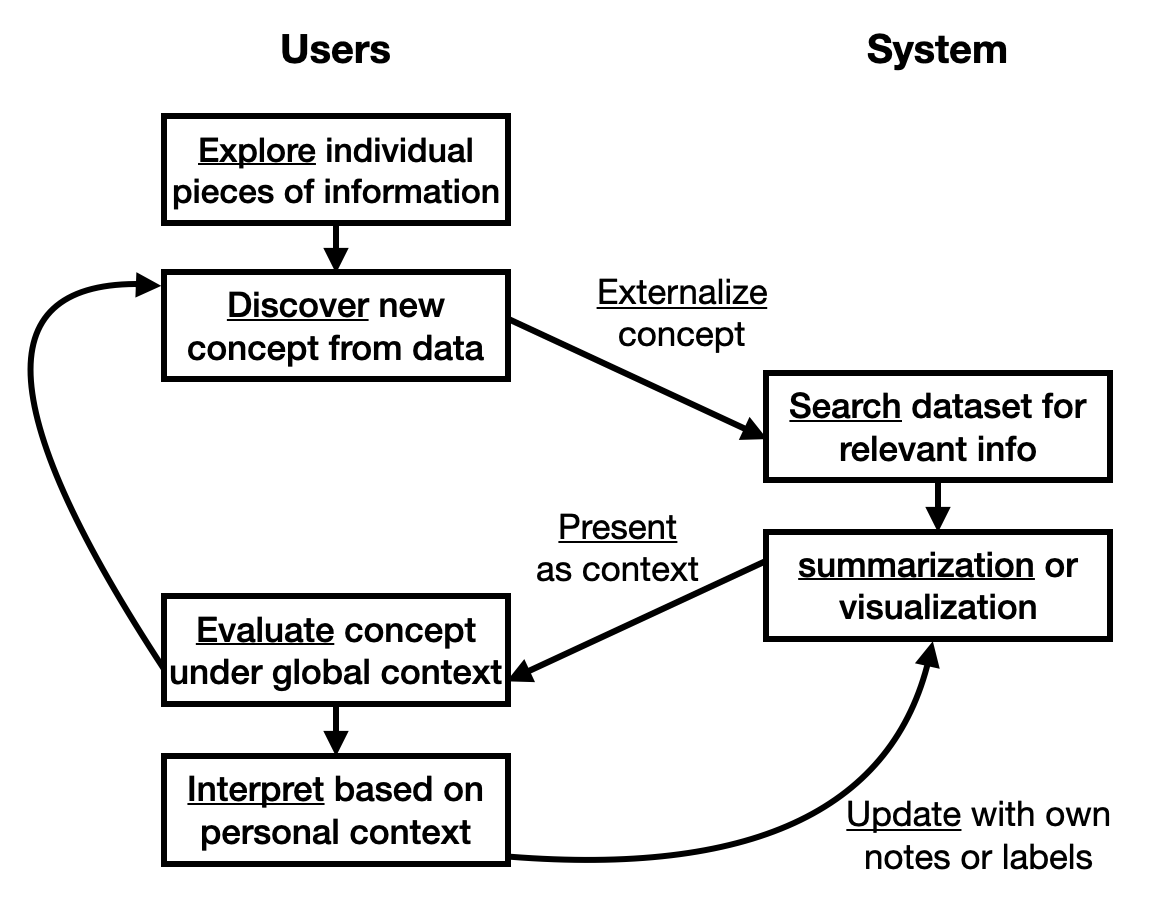
\includegraphics[width=0.6\textwidth]{images/framework.png}
    \caption[A general system design pattern.]{A general system design pattern.}
    \label{fig:framework}
\end{figure}


In general, the systems described in this dissertation followed the above sensemaking design pattern that aimed to provide better support for global context during bottom-up exploration of large and unstructured data. The framework starts with users \textbf{exploring} individual pieces of information in the dataset. For individuals, this is typically the initial queries when conducting online exploratory searches with Yelp, Google or Amazon as in \Cref{chap:searchlens,chap:weaver,chap:mesh}, respectively. Similarly, the crowd system Alloy (\Cref{chap:alloy}) simulated this process by allowing workers to repeatedly sample from the datasets to iteratively build up a better understanding of the space of information. As users process the individual pieces of evidence, they \textbf{discover} concepts that were important to their task. In the case of Alloy, this would be crowdworkers identifying categories to for organizing items in the dataset; in the case of SearchLens and Mesh, this would be individuals identifying criteria from a restaurant or product review that fits users’ personal interests; and in the case of Weaver, this would be users identifying a restaurant or travel destination on a webpage. 

Since the users often discovered useful concepts from examining a single piece of information, it can be difficult for them to evaluate such concepts under the global context without spending significant effort. For example, a consumer comparing products may find a recommendation on one webpage but wonder whether other websites also recommend it. Reading the review she might discover useful criteria about the type of product she is researching, but figuring out how all the different options performed for that specific criteria can be very high costs, requiring her to go through many reviews for each option. Motivated by this need, users then \textbf{externalize} newly identified concepts to the systems to access relevant information across the entire dataset. In the case of Alloy, crowdworkers highlighted keywords in the sampled items to search for other items across the dataset to group them into the same categories; in the cases of SearchLens and Mesh, users used keywords they identified in reviews as criteria to search for reviews across different restaurants on Yelp or products on Amazon; and in the case of Weaver, users simply hover over an entity mention to express interests to the system. 

The system in turn used the keywords or entity mentions to \textbf{search} across the entire dataset (i.e., text items in a dataset in Alloy, reviews of different options in SearchLens and Mesh, or text snippets across different browser tabs in Weaver), and \textbf{summarizes} the search results to provide concept-specific global context to the users. In the systems presented in this dissertation, this included directly showing a list of search results in Alloy, showing the average ratings of reviews that mentioned a specific criteria in Mesh, and presenting visual explanations for each search result in SearchLens. In addition to the summarizations, all systems also allowed its users to drill-down and explore each item in the search results which often leads to new iterations of discovering and externalizing new concepts for further investigation forming a discovery-exploration loop.

Evaluation results presented in \Cref{chap:alloy} showed that the same clustering algorithm performed better when only using keywords selected by the crowdworkers when compared to using all words as features. This showed that crowdworkers were capable of selecting discriminatory keywords to represent the categories. Based on this insight, I continued to use this strategy of allowing users to externalize their mental concepts (i.e., criteria) in systems that supported individual online sensemaking later in this document. Admittedly, document search algorithms still make occasional mistakes, and it is important to provide mechanisms to the users to recover from system errors. For this, users can \textbf{update} the summaries generated by the systems to better reflect their own interpretation of data. In the case of Alloy, crowdworkers labeled each item in the search results to indicate whether they should be in the same category or not; in the case of Mesh, individuals can change the average rating based on their own judgement after reading the reviews. This pattern is especially important when the summaries themselves are the final artifacts for users such as in Alloy (labeling items with categories) and Mesh (generating a personalized product comparison table).


\section{Conclusion}

Bottom-up exploration of large quantities of unstructured information is ubiquitous, but it can also be challenging to users due to the individual's limited capacity to understand global context throughout the exploration. Crowdsourcing is one example of this where each crowdworker’s capacity to process data is further limited by the scope of microscopes, and the requesters often turn to crowdsourcing for scale and do not have the capacity to understand their own datasets fully. Another example is consumer research, where users are faced with making decisions based on their personal interpretation of an enormous amount of online evidence about many different choices.  

In this dissertation, I investigated the core thesis of providing global context during bottom-up data exploration by designing and building five novel systems and interaction techniques. The key insight is that users need global context that reflects their evolving interests to support sensemaking throughout their exploration. Through extensive lab and field studies, I demonstrated benefits to users over existing approaches, include allowing users to identify patterns in data and propose categories at the right abstraction level under the global context (\Cref{chap:alloy}), identify \emph{residue} and improve current schema \Cref{chap:revolt}, evaluate new concepts based on current interests under global context \Cref{chap:searchlens,chap:weaver}, and evaluate newly discovered criteria to prioritize research efforts \Cref{chap:mesh}. Better support for bottom-up data exploration is likely to become increasingly important these two scenarios explored in this document:  For crowdsourcing, modern machine learning models demand increasingly large amounts of high quality training labels; and for individual online research, the rise of online misinformation and shill reviews makes traditional automated aggregation techniques that increasingly vulnerable. This thesis introduced novel interaction paradigms and insights about how users can benefit from them, as well as a general design pattern that can inform the building of future systems that can support global context during bottom-up data exploration.
